\documentclass[12pt]{article}

\usepackage{fullpage}
\usepackage{multicol,multirow}
\usepackage{tabularx}
\usepackage{ulem}
\usepackage{hyperref}
\usepackage{graphicx}
\usepackage[utf8]{inputenc}
\usepackage[russian]{babel}

\begin{document}

\section*{Лабораторная работа №\,1 по курсу дискрeтного анализа: сортировка за линейное время}

Выполнил студент группы М8О-207БВ-24 МАИ \textit{Устинов Александр}.

\subsection*{Условие}
 
\begin{enumerate}
\item Общая постановка задачи.
Требуется разработать программу, осуществляющую ввод пар «ключ-значение», 
их упорядочивание по возрастанию ключа алгоритмом "Сортировка подсчетом" за 
линейное время и вывод отсортированной последовательности. 

\item Вариант задания.
Тип ключа: почтовые индексы.
Тип значения: строки переменной длины (до 2048 символов).
\end{enumerate}

\subsection*{Метод решения}

Для решения задачи был использован алгоритм "Сортировка подсчетом" (Counting Sort), который позволяет сортировать целочисленные ключи за линейное время при условии,
что диапазон ключей не слишком велик. Поскольку почтовые индексы представляют собой 6-значные числа, алгоритм эффективен для данной задачи.

\begin{enumerate}
\item Создается массив счетчиков размером значения максимального ключа + 1.
\item Проход по входным данным для подсчета количества вхождений каждого ключа.
\item Вычисление префиксных сумм для определения позиций ключей в отсортированном массиве.
\item Создание выходного массива и заполнение его на основе подсчитанных позиций.
\end{enumerate}

\textbf{Архитектура программы:}

\begin{center}
\begin{tabular}{@{}l@{}}
\texttt{main.cpp} \\
\quad $\vdash$ \textbf{Ввод данных} --- чтение из stdin \texttt{<ключ>\textbackslash t<значение>} \\
\quad $\vdash$ \textbf{Структура \texttt{Entry}} --- ключ, ключ-строка, значение \\
\quad $\vdash$ \textbf{Функция \texttt{CountingSortEntries}} --- сортировка за $O(n + k)$ \\
\quad $\vdash$ \textbf{Вывод} --- записи в stdout в исходном формате \\
\end{tabular}
\end{center}

\vspace{0.3cm}


\textbf{Использованные источники:}
\begin{itemize}
\item Кормен Т., Лейзерсон Ч., Ривест Р., Штайн К. ``Алгоритмы: построение и анализ''.
\item \url{https://en.wikipedia.org/wiki/Counting\_sort}
\end{itemize} 

\subsection*{Описание программы}

Программа реализована в 1 файле main.cpp

Описание основных типов данных:
\begin{enumerate}
\item \texttt{struct Entry} — структура для хранения пары ключ-значение, где ключ представлен как целое число и строка (для сохранения ведущих нулей), а значение — строка переменной длины.
\item \texttt{std::vector<Entry>} — динамический массив для хранения всех записей, считанных из входного потока.
\item \texttt{std::vector<uint32\_t>} — массив счетчиков для алгоритма сортировки подсчетом, где индекс соответствует ключу, а значение — количеству его вхождений.
\end{enumerate}

Описание основных функций:
\begin{enumerate}
\item \texttt{CountingSortEntries} — функция, реализующая алгоритм сортировки подсчетом для массива записей. Она принимает вектор записей и возвращает отсортированный вектор.
\item \texttt{main} — основная функция, которая читает входные данные, вызывает функцию сортировки и выводит результат.
\end{enumerate}

\subsection*{Дневник отладки}

\begin{enumerate}
\item Массив result создавался размером max\_val + 1, из-за чего в выводе появлялись лишние нули.

Решение: размер изменен на keys.size()

\item Ключ 000000 выводился как 0, так как хранился только как число.

Решение: добавлено поле key\_str для сохранения исходного представления ключа.

\item Ввод завершался при первой пустой строке.

Решение: пустые строки теперь пропускаются через continue, а не завершают ввод.

\item vector<size\_t> на большое количество элементов занимал слишком много памяти + было копирование строк.

Решение: Замена на vector<uint32\_t> + std::move для строк.

\item Вложенный цикл для сопоставления отсортированных ключей с записями.

Решение: Сортировка записей напрямую в функции CountingSortEntries за $O(n + k)$.

\item Цикл начинался с $i$ = keys.size(), что приводит к обращению по несуществующему индексу.

Решение: Исправлено на $i$ = keys.size() - 1.
\end{enumerate}

\subsection*{Тест производительности}

Для проверки было проведено 4 теста: входные данные содержали 1000, 10000, 100000 и 1000000 записей.
Время выполнения было измерено с помощью функции std::chrono.
Результаты показали, что время выполнения растет примерно линейно с увеличением количества записей, что соответствует теоретической сложностной оценке алгоритма $O(n + k)$.

\begin{figure}[h]
\centering
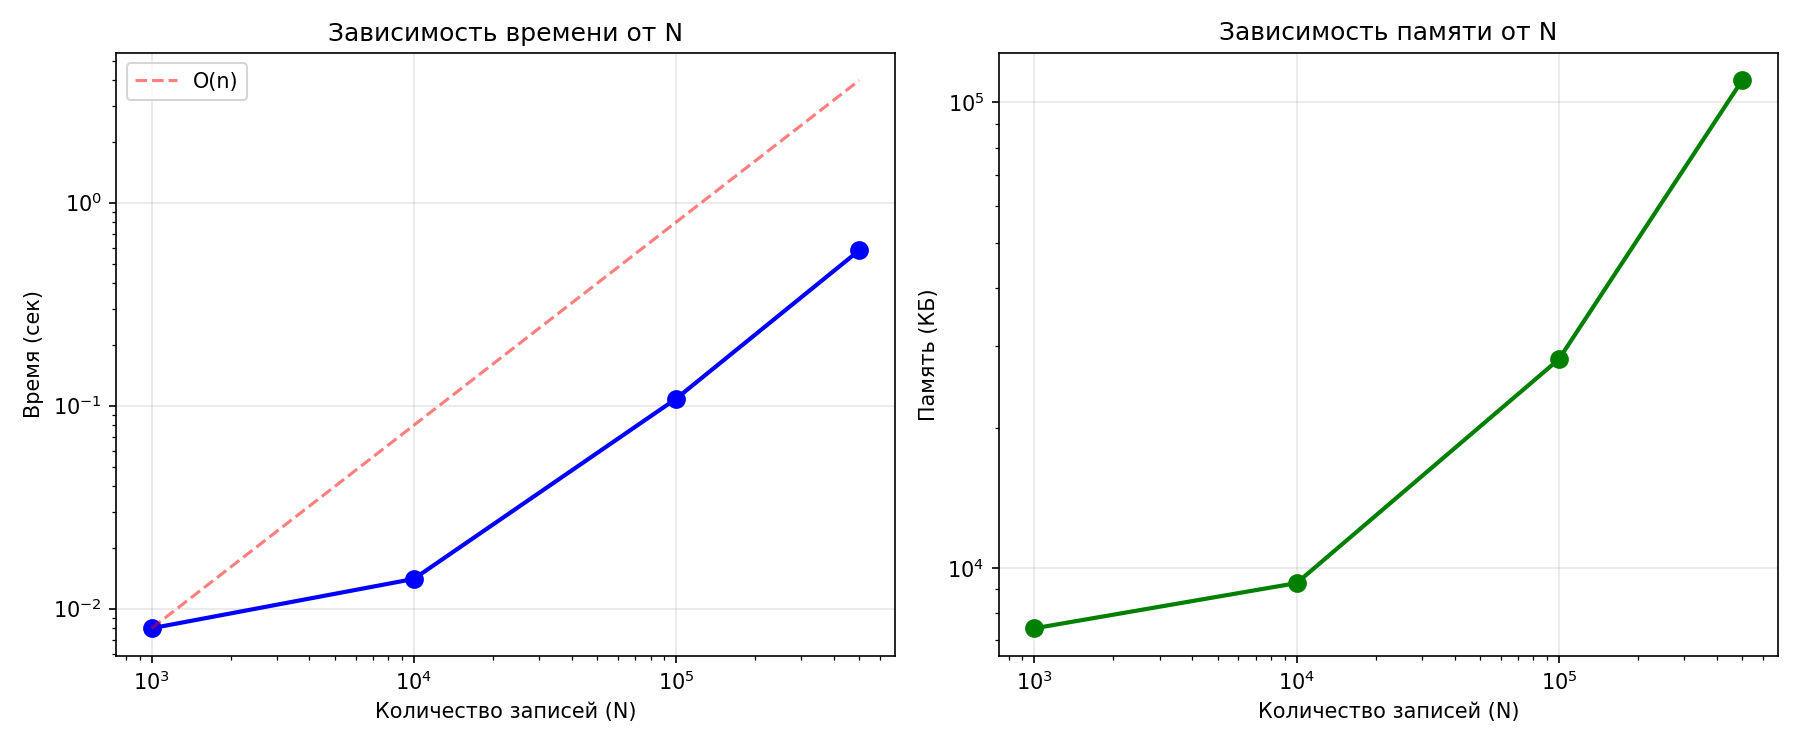
\includegraphics[width=0.8\textwidth]{benchmark.png}
\caption{Результаты тестирования производительности}
\label{fig:benchmark}
\end{figure}

График тестов сохранен в файле benchmark.png. Код для построения графика написан в benchmark.py

\subsection*{Недочёты}

\begin{enumerate}
\item Массив счётчиков требует $O(k)$ памяти,
где $k$~--- максимальный ключ. Для почтовых индексов (до 999999) это примерно 4~МБ.

Почему не исправлено: это фундаментальное ограничение алгоритма

\item При вводе нечисловых символов в ключе std::stoi() выбрасывает исключение. Не добавлена проверка на корректность преобразования.

Почему не исправлено: по ТЗ предполагается, что входные данные корректны.
\end{enumerate}


\subsection*{Выводы}

Сортировка подсчётом эффективна для сортировки целочисленных ключей в ограниченном диапазоне, когда требуется линейная сложность и стабильность. 
Типовые задачи: сортировка почтовых индексов, ID-номеров, символов, а также использование в качестве подпрограммы в поразрядной сортировке.

Сложность программирования — средняя. Алгоритм прост в реализации (около 30 строк кода), но требует внимательности при работе с граничными индексами и оптимизации памяти.

Возникшие проблемы: выход за границы массива в циклах, потеря ведущих нулей в ключах (решено хранением строкового представления), высокое потребление памяти (решено заменой \texttt{size\_t} на \texttt{uint32\_t}),
квадратичная сложность при сопоставлении ключей (решено сортировкой записей напрямую).
Все проблемы успешно устранены, программа соответствует требованиям ТЗ.

\end{document}